%! TeX program = xelatex
%! TEX TS-program = xelatex
\documentclass[11pt,a4paper,titlepage]{article}

% Language
\usepackage{polyglossia}
\setdefaultlanguage[frenchpart=false, frenchfootnote=true, frenchitemlabels=true]{french}
\usepackage{numprint}

% Fonts
\usepackage{fontspec}
\setmainfont{Linux Libertine O}
\setsansfont{Linux Biolinum O}

\usepackage{mathtools}
\usepackage{amssymb}
\usepackage{amsfonts}
\usepackage{graphicx}
\usepackage{float}
\usepackage{listings}
\usepackage{hyperref}
\usepackage{attachfile2}
\usepackage{vhistory}
\usepackage{epsfig}

\usepackage{fullpage}
\usepackage[parfill]{parskip}

\usepackage{xcolor}

%-----------------------------------------------------------

\newcommand{\up}[1]{\textsuperscript{#1}}
\newcommand{\down}[1]{\textsubscript{#1}}

\newcommand{\addcode}[3]{
    \begin{figure}[H]
        \centering
        \lstinputlisting[language=#2, caption=\textattachfile{#1}{#1}, label=#3]{#1}
    \end{figure}
}

\newcommand{\addimg}[4]{
    \begin{figure}[H]
        \centering
        \includegraphics[#2]{#1}
    \caption{#3}
    \label{#4}
    \end{figure}
}

%-----------------------------------------------------------

\definecolor{base}{RGB}{250,245,237}
\definecolor{subtle}{RGB}{110,107,135}
\definecolor{red}{RGB}{181,99,122}
\definecolor{gold}{RGB}{235,158,51}
\definecolor{rose}{RGB}{214,130,125}
\definecolor{pine}{RGB}{41,105,130}
\definecolor{foam}{RGB}{87,148,158}
\definecolor{iris}{RGB}{143,122,168}

\hypersetup{
    colorlinks=true,
        allcolors=iris
}
\attachfilesetup{color=iris}

%-----------------------------------------------------------

\lstset{
    % backgroundcolor=\color{white},        % background color
        basicstyle=\ttfamily,                   % regular style
        breakatwhitespace=true,                 % sets if automatic breaks should only happen at whitespace
        breaklines=true,                        % sets automatic line breaking
        captionpos=t,                           % caption-position
        commentstyle=\itshape\color{subtle},    % comment style
        % deletekeywords={...},                 % delete keywords from the given language
        escapeinside={\%*}{*)},                 % if you want to add LaTeX within your code
        firstnumber=1,                          % start line enumeration with line 1
        frame=tb,                               % adds a frame around the code
        keepspaces=true,                        % keeps spaces in text
        keywordstyle=\color{pine},              % keyword style
        language=C++,                           % language of the code
        % morekeywords={*,...},                 % add more keywords to the set
        numbers=left,                           % position of line-numbers; possible values are (none, left, right)
        numbersep=15pt,                         % distance between line-numbers and the code
        numberstyle=\scriptsize\ttfamily\color{subtle}, % style used for line-numbers
        % rulecolor=\color{black},              % if not set, the frame-color may be changed on line-breaks within not-black text (e.g. comments (green here))
        showspaces=false,                       % show spaces everywhere
        showstringspaces=false,                 % underline spaces within strings only
        showtabs=false,                         % show tabs within strings
        stepnumber=1,                           % step between two line-numbers
        stringstyle=\color{red},               % string literal style
        tabsize=4,	                          % default tabsize
        % title=\lstname                        % show the filename
}

%-----------------------------------------------------------

\title{{\Huge Quoridor\\ }Software Requirement Document}
\author{Francesco Nieri \and Boris Petrov \and Nargis Sghiouar \and Elizabeth Jankovic \and Sacha Testaert \and Elias Ibnoussina \and Louis Vanstappen \and Anne-Marie Kourieh}
\date{\today}

\pagebreak

\begin{document}
\maketitle
\tableofcontents

%-----------------------------------------------------------

\section{Introduction}

Quoridor est un jeu se jouant sur un plateau avec des pions et des murs à 2 ou 4 joueurs.
Les règles de jeu sont disponibles \href{http://www.gigamic.com/files/catalog/products/rules/quoridor-classic-fr.pdf}{ici}.

Lors de ce projet, nous allons créer une partie serveur gérant le jeu, le chat, et toutes autres fonctionnalités liées à la gestion d'amis et utilisateur.

Nous allons aussi créer un programme client permettant à un utilisateur de jouer à Quoridor, ainsi que de réaliser toute autre action en communiquant avec le serveur. Le client offre une interface graphique interactive. Le client sera tout d'abord exclusivement utilisable sur le terminal. Il sera ensuite accessible via une GUI. Il est important de noter que la GUI et le terminal auront les mêmes fonctionnalités, leurs différences se résumeront à l'aspect cosmétique.

Dans ce document, nous allons élaborer les besoins que nous estimons important pour l'accomplissement de ce programme.

\newpage
\subsection{Historique}
\begin{versionhistory}
    \vhEntry{0.0}{19/11/2021}{Boris Petrov}{Creation du SRD.}
    \vhEntry{0.1}{23/11/2021}{Boris Petrov}{Ajout des besoins système.}
    \vhEntry{0.2}{23/11/2021}{Francesco Nieri}{Ajout du calcul ELO et fonctionnement du système.}
    \vhEntry{0.3}{23/11/2021}{Louis Vanstappen et Elizabeth Jankovic}{Ajout des besoins système non fonctionnels, design du système.}
    \vhEntry{0.4}{23/11/2021}{Boris Petrov}{Correction besoins fonctionnels.}
    \vhEntry{0.5}{23/11/2021}{Nargis Sghiouar et Anne-Marie Kourieh}{Ajout des besoins utilisateur.}
    \vhEntry{0.6}{24/11/2021}{Boris Petrov}{Diverses modifications à la structure du SRD (Placeholders, readme, main).}
    \vhEntry{0.7}{24/11/2021}{Elias Ibnoussina et Sacha Testaert}{Ajout besoins utilisateur non fonctionnels.}
    \vhEntry{0.8}{24/11/2021}{Francesco Nieri}{Ajout de l'historique.}
    \vhEntry{0.9}{24/11/2021}{Elizabeth Jankovic}{Ajout des modalités de jeu supplementaires.}
    \vhEntry{0.10}{24/11/2021}{Louis Vanstappen}{Ajout de l'introduction, correction des fautes.}
    \vhEntry{0.11}{07/12/2021}{Francesco Nieri}{Modifications au diagramme de classe de l'utilisateur}
    \vhEntry{0.12}{9/12/2021}{Boris Petrov}{Ajout de détails sur la gestion d'une partie}
    \vhEntry{0.13}{9/12/2021}{Elizabeth Jankovic}{Ajout du diagramme des cas d'utilisations du côté serveur}
    \vhEntry{0.14}{10/12/2021}{Louis Vanstappen}{Description des choix possibles de bases de données}
    \vhEntry{0.15}{10/12/2021}{Francesco Nieri}{Amélioration du diagramme à propos du chat}
    \vhEntry{0.16}{10/12/2021}{Louis Vanstappen}{Correction de petites erreurs et d'orthographe}
    \vhEntry{0.17}{12/12/2021}{Francesco Nieri}{Réécriture des besoins utilisateurs non fonctionnels}
    \vhEntry{0.18}{13/12/2021}{Francesco Nieri}{Correction des mélanges entre français et anglais dans les diagrammes et dans le phrases du SRD}
\end{versionhistory}



\section{Besoins Utilisateur: Fonctionnels}

\subsection{Connexion}
    Avant de pouvoir jouer, l'utilisateur doit se connecter. Si l'utilisateur ne possède pas de compte, il doit s'en créer un. Pour cela, il choisit un pseudonyme et un mot de passe à retenir. 

\subsection{Menu principal}
\addimg{img/2_UseCaseGame.eps}{width=\linewidth}{Use Case Menu}{usecasemenu}

\subsubsection{Gérer une liste d'amis}
    Chaque utilisateur dispose d'une liste d'amis. Quand il ajoute ou supprime un ami, les modifications se verront sur cette liste que l'utilisateur peut consulter. Pour ajouter un ami, il suffit de connaître son pseudonyme et d'attendre qu'il accepte sa requête. 
    
\subsubsection{Chat}
    Pour discuter avec ses amis, il choisit des amis dans sa liste d'amis et écrit son message. Ainsi, un joueur peut discuter avec ses amis même lors d'une partie. L'utilisateur peut également quitter une discussion. 
    
\subsubsection{Consulter le classement}
    Un score est attribué à chaque joueur. Tous les utilisateurs existants sont recensés et classés selon leurs performances de jeu. Il est possible de consulter ce classement.

\subsubsection{Lancement d'une partie}
    L'utilisateur a le choix de démarrer une nouvelle partie, d'en rejoindre une ou de reprendre une partie sauvegardée. Lors de la création d'une nouvelle partie, l'utilisateur configure les paramètres, c'est-à-dire précise le mode de jeu et le nombre de joueurs. Il a la possibilité d'inviter des amis s'il le souhaite.



\subsection{Au cours d'une partie}
\addimg{img/2_UseCaseMenu.eps}{width=\linewidth}{Use Case Game}{usecasegame}
    \subsubsection{Faire un mouvement}
    Quand c'est au tour de l'utilisateur de jouer, il va devoir soit placer un mur, soit déplacer son pion sur l'une des quatre cases voisines. 
    \subsubsection{Sauvegarder}
    Les joueurs peuvent mettre en pause et sauvegarder la partie actuelle en demandant l'accord aux autres joueurs.
    \subsubsection{Abandonner}
    Pendant une partie, l'utilisateur peut également la quitter. Ainsi, il sera perdant.


\section{Besoins Utilisateurs : Non Fonctionnels}
\begin{itemize}
	\item Les informations sensibles de l'utilisateur sont stockées de manière sécurisée
	\item L'interface est intuitive et octroie une liberté d'action quant à ce que l'utilisateur désire faire
	\item Interagir avec ses amis et adversaires
	\item Le système est suffisament réactif que pour ne pas sortir le joueur de sa partie
\end{itemize}

\section{Besoins système fonctionnels}
\subsection{Connexion}

L'accès au fonctionnalités du système ne doit être accordé
qu'aux utilisateurs ayant fourni un nom d'utilisateur (ou
\emph{username}) et un mot de passe (ou \emph{password})
corrects. Ceux-ci sont corrects s'ils correspondent
 à une entrée dans la base de données.

Le système doit donc pouvoir confirmer les identifiants
grâce à une requête au serveur depuis
la machine de l'utilisateur.
Si la partie client ne parvient pas à établir une connexion
avec la partie serveur,
le système doit pouvoir en informer
l'utilisateur et refuser toute tentative de connexion.
% Tous deux doivent être composés de caractères
% alphanumériques.

Le système doit pouvoir donner l'occasion à l'utilisateur d'entrer
ses informations grâce à un formulaire ou une demande
séquentielle. Si les informations entrées ne sont pas
correctes, le système doit pouvoir communiquer à
l'utilisateur un message d'erreur utile et lui laisser la
possibilité d'essayer à nouveau.

\addimg{img/4_LogActivity.eps}{width=\linewidth/5*3}{Étapes lors d'une connexion}{log_proc}

% Si l'utilisateur ne se souvient plus de son nom
% d'utilisateur ou de son mot de passe, le
% système doit pouvoir lui fournir un moyen de regagner accès
% à son compte.

% \subsubsection{Regain d'accès au compte utilisateur}

% Un courriel de récupération contenant le nom d'utilisateur et un
% hyperlien renvoyant vers une page permettant le changement
% du mot de passe doit pouvoir être envoyé
% dans le cas d'un
% oubli d'identifiants.

% Le mot de passe étant chiffré par un processus irréversible dans la base
% de données, seul un nouveau mot de passe permet un regain
% d'accès.

% Le processus de changement de mot de passe doit rendre
% l'ancien mot de passe invalide et rendre le nouveau mot de
% passe l'unique clé d'accès au compte associé.

\subsection{Gestion des comptes}


% Un compte doit être identifié grâce à une adresse courriel
% et un nom d'utilisateur.

Un compte doit être identifié grâce au nom d'utilisateur. 
Chaque compte doit être unique et par conséquent,
deux comptes différents ne peuvent pas avoir
les mêmes identifiants. Le système doit pouvoir accéder aux
identifiants séparément ou en lot.

Le mot de passe, bien qu'essentiel au compte, ne doit pas
faire
partie de son identité. Deux comptes différents
peuvent avoir le même mot de passe.

Les informations relatives aux comptes des utilisateurs
doivent être stockées dans une base de données centrale et
accessibles depuis chaque client \emph{via} Internet.

\subsubsection{Création de compte}

Si un visiteur du système ne possède pas de compte
utilisateur, le système doit pouvoir lui donner la
possibilité d'en créer un.

Durant ce processus, le système doit pouvoir demander au
visiteur~: un nom d'utilisateur et un
mot de passe. Le système doit s'assurer que le
premier champ n'existe pas déjà dans la base de données.
Si c'est le cas, le système doit refuser la demande
d'inscription et en informer le visiteur.

% Si les identifiants sont tous deux uniques, le système doit
% pouvoir envoyer un courriel de confirmation à l'adresse
% courriel fournie. Le compte ainsi créé ne sera actif qu'à
% partir de la confirmation de l'adresse courriel par le
% visiteur et deviendra dès lors un utilisateur.

\subsubsection{Suppression de compte}

Le système doit donner l'opportunité à tout utilisateur de
supprimer son compte. Ce processus de suppression se solde
par une suppression définitive et irrévocable du compte
associé dans la base de données.
Les identifiants qui étaient utilisés par ce
dernier doivent être de nouveau disponibles pour de
nouvelles inscriptions.

Le système ne doit supprimer en aucun cas un compte
utilisateur sans la confirmation de son titulaire.

\subsection{Menu principal}

Le menu principal du système doit pouvoir donner accès aux
actions suivantes à tout utilisateur authentifié~:

\begin{itemize}
    \item jouer~;
    \item consulter les classements~;
    \item discuter avec ses amis~;
    \item modifier ses informations personnelles.
\end{itemize}

\subsection{Interactions entre utilisateurs}

Le système doit donner la possibilité à chaque utilisateur
authentifié de gérer une liste d'amis. L'utilisateur doit
pouvoir ajouter des amis et en supprimer. L'ajout se
fait au moyen de demandes d'ami que tout utilisateur peut
envoyer à tout autre utilisateur à condition qu'il connaisse
son nom d'utilisateur.

Ces listes d'amis sont stockées dans la base de données et
propres à chaque utilisateur, personne d'autre que
l'utilisateur authentifié ne devrait y avoir accès.

\subsubsection{Discuter avec ses amis}


Le système doit donner la possibilité à tout utilisateur
authentifié de discuter avec ses amis par messages écrits
dans des fils de discussion privés.

% Le système doit
% également offrir la possibilité aux utilisateurs de créer
% des groupes de discussion où plusieurs utilisateurs
% peuvent participer. Les participants doivent pouvoir être
% ajoutés soit lors de la création du groupe, soit après
% celle-ci par tout participant du groupe grâce à un système
% d'invitations.

Tout message envoyé sur ces fils de discussion doit être
sauvegardé dans la base de données dès son envoi,
visible par tous les
participants et supprimable par son auteur. Les messages
doivent être persistants d'une session à l'autre.

Pour pouvoir supprimer les messages individuellement, ces
derniers doivent posséder un identificateur unique composé
notamment de l'heure d'envoi et de l'expéditeur.

\subsection{Consulter les classements}

Tout utilisateur doit avoir un score qui indique son niveau
au jeu. Ce score est modifié à l'issue de chaque partie
par le système d'évaluation \emph{ELO}.

Le système doit pouvoir, grâce à ce score, constituer
un classement des meilleurs utilisateurs. Ce classement doit
pouvoir être visible par tout utilisateur authentifié du système.

Ce classement doit être consultable et filtrable.
L'utilisateur doit avoir la possibilité d'afficher
soit totalité des utilisateurs, soit uniquement les utilisateurs
amis.

\subsection{Modifier ses informations personnelles}

Le système doit fournir la possibilité à tout utilisateur de
modifier ses informations personnelles. Cela inclut 
le nom d'utilisateur et le mot de passe.
La modification de chacune de ces informations doit être
définitive et la nouvelle valeur doit être
sauvegardée dans la base de données.

\subsection{Jouer}

Pour jouer, l'utilisateur doit initialiser une recherche
d'adversaire pour le mode de
jeu qu'il a choisi. Cette étape est ce qu'on appelle le
\emph{matchmaking}. Le système doit s'assurer que les
utilisateurs choisis pour une partie aient choisi le même
mode de jeu.
% Le système doit s'assurer que lorqu'un
% match est prêt à être lancé, les deux utilisateurs choisis soient
% toujours connectés.

\subsubsection{Matchmaking}

Lorqu'un joueur entre dans le matchmaking, il doit être
placé dans une file d'attente à priorité.
La priorité de chaque joueur est définie selon la durée
écoulée
depuis son entrée dans le matchmaking. Cette durée est dite \emph{temps d'attente}.
Pour séparer les modes de jeu, le système doit gérer une
file d'attente distincte pour chaque mode de jeu.

Le choix d'un adversaire adéquat doit ainsi dépendre de son temps
d'attente mais aussi, et surtout, de son \emph{ELO}.
À l'issue d'une situation optimale, les deux utilisateurs doivent
avoir un \emph{ELO} similaire et avoir eu un temps d'attente presque
nul.

Chaque utilisateur doit avoir la possibilité de voir le nombre d'utilisateurs
dans la file d'attente ainsi que son temps d'attente. Le
système doit lui donner la possibilité de quitter le
matchmaking.

Un utilisateur dans le matchmaking doit y être est enlevé
dès qu'il y a trouvé un adversaire, que sa connexion au
serveur n'est plus valide ou qu'il a quitté la file
d'attente de son plein gré.

\subsubsection{Partie de Quoridor}

Lors d'une partie, le système doit faire une distinction
entre les actions disponibles aux participants en tant que
\emph{joueurs}, et
celles disponibles en tant qu'\emph{utilisateurs}.

Un joueur est celui qui fait des actions sur le
plateau de jeu, alors qu'un utilisateur fait des
actions en-dehors du plateau de jeu. Le joueur ne peut agir
que lorsque c'est son tour de jouer alors que l'utilisateur, au
contraire, peut agir tout le temps.

Les actions du joueur seraient de déplacer un pion
et de placer un mur alors que celles de l'utilisateur
seraient de discuter avec des amis, déclarer forfait,
etc.

Le système doit permettre aux participants de jouer,
chacun à leur tour, jusqu'à une victoire potentielle
de l'un des deux. Les règles du jeu étant telles que
des parties nulles sont impossibles.

Lors d'une fin de partie, le système doit en informer les
participants, mettre à jour l'\emph{ELO} de chaque
utilisateur et renvoyer les utilisateurs vers le menu principal.

Il est à noter que plusieurs parties en parallèle doivent être
possibles sur le serveur, chacune ayant lieu indépendamment des
autres et n'ayant aucune connaissance de celles-ci.

\addimg{img/4_TurnActivity.eps}{width=\linewidth/5*4}{Étapes lors d'un tour}{log_proc}

\subsubsection{Gestion d'une partie de Quoridor}

Le système doit pouvoir gérer deux plateaux distincts.
Celui des pions et celui des murs. Les plateaux
doivent être gérés par un contrôleur commun puisqu'ils
sont dépendants l'un de l'autre.

% Création d'une partie, matchmaking
% Gestion d'une partie, gestion murs, gestion pions, gestion
% score, gestion vainqueur
% Mise à jour du classement




\section{Notre jolie game diagramme (prend moi ça Boris)}

Le jeu est divisé en deux plateaux. Le plateau mur (Wall board) contient les murs. Alors que le plateau joueur contient les pions des
joueurs. Chaque pion a une couleur différente afin de permettre aux joueurs de se différencier l'un de l'autre. La classe board combine
chaque plateau, qui sera ensuite afficher par BoardPrinter dans MainWindow. 

Le PlayerBoard est divisé en cases. Chaque case peut accueillir au maximum un pion définit par la classe Player. Chaque Player peut
se déplacer sur le PlayerBoard en faisant appel à la classe PlayerAction, qui vérifie si le coup est valide.

Le WallBoard est quant à lui est divisé en couloir. Chaque couloir peut contenir un Wall. Un couloir a une largeur de 2 cells. L'utilisateur
peut placer un wall en faisant appel à WallAction qui va d'abord vérifier si l'action est valide.

\section{Partie 5: Besoin système non fonctionnels}
\subsection{Système d'exploitation}
Le programme doit être capable de tourner sous Linux, plus précisément avec la distribution Ubuntu 20.04 même s'il devrait savoir tourner
sur n'importe quelle autre distribution.
Ce serait potentiellement justifié de créer une version Windows et MacOS, mais ce n'est pas une priorité.

\subsection{Réseau}
Le programme va faire l'utilisation de socket pour permettre la communication entre le serveur et le client. 
Le client devra éventuellement faire des requêtes vers des APIs externes.

\subsection{Disponibilité}
Afin que le programme fonctionne correctement, il est primordial que le serveur soit disponible, c'est à dire existant et accessible. 

\subsection{Performance}
Étant donné que le programme ne nécessite pas une grande performance graphique et que les calculs de jeu sont effectués sur un serveur, le
programme est propice à avoir une bonne performance. Il faut s'assurer que les calculs exécutés sur le serveur soit effectués le plus
rapidement possible afin de renvoyé une réponse au client le plus rapidement possible. Le jeu doit pouvoir être joué rapidement, il faut
donc réduire au maximum le temps d'attente entre chaque coup.
Il faut aussi que le programme utilise 2 threads, un pour l'affichage graphique et un pour les requêtes asynchrones, afin d'éviter que le
programme ne sache plus réagir aux input du client.

\subsection{Capacité}
Le client doit avoir la capacité de lire des données du serveur et de les afficher à l'utilisateur. Il doit aussi être capable de gérer les
entrées de l'utilisateur et d'en faire part au serveur.

Le serveur doit avoir la capacité de gérer chaque calcul lié au jeu, par exemple vérifié qu'un coup est valide. Il doit aussi être capable
de manipuler dans une base de données le chat, les données en rapport au jeu, tel que l'état de la partie en cas de sauvegarde, et les 
données utilisateurs.

\subsection{Sécurité}
Afin d'être correctement sécurisé, le programme va encrypter les mots de passe avant des les enregistrer dans la base de données avec un
algorithme de hashing, tel que SHA-256. Une salt key sera aussi utilisée lors de l'encryption pour amélioré la sécurité.

Il peut aussi s'avérer utile d'établir une socket sécurisé à l'aide d'un certificat SSL. Cela permettrait entre autre de communiquer par HTTPS au
lieu que par HTTP.

\subsection{Robustesse}
Le client doit être capable de résister à tout input de l'utilisateur sans cracher.
Le serveur doit savoir gérer n'importe quel type de requêtes sans crash. Il doit aussi être capable de limiter ses actions au bon utilisateur.

\section{Partie 6: Design et fonctionnement du système}
\subsection{fonctionnement du système}
\subsubsection{Boucle du jeu: Client}
\begin{itemize}
    \item Flow of a game (use activity diagram made by Boris)

        À chaque tour, le client va envoyer une requête au serveur. Si le jeu est terminé, le serveur renverra un message au client pour que
        celui-ci puisse arrêter la boucle de jeu.
    \item Chat

        Le chat se met à jour à chaque fois que le serveur envoie un message au client. Et un player écris un message qui est envoyé au serveur.
\end{itemize}
\subsubsection{Boucle du jeu: Serveur}
\begin{itemize}
    \item Jeu

        Lorsque le client joue un coup, le serveur va vérifier que ce coup est valide et que la partie n'est pas fini. Il informera ensuite
        le client.

    \item Chat
    
        Le serveur doit informer les clients lorsque un message a été envoyé dans le chat.


\end{itemize}

\subsection{Design du système}
    Le système se dècoupe essentiellement en 3 parties:
    \begin{itemize}
        \item[-] Coté utilisateur
        \item[-] Coté jeu
        \item[-] Coté Server   
    \end{itemize}
    \subsubsection{Coté utilisateur}
        % \makebox[\textwidth]{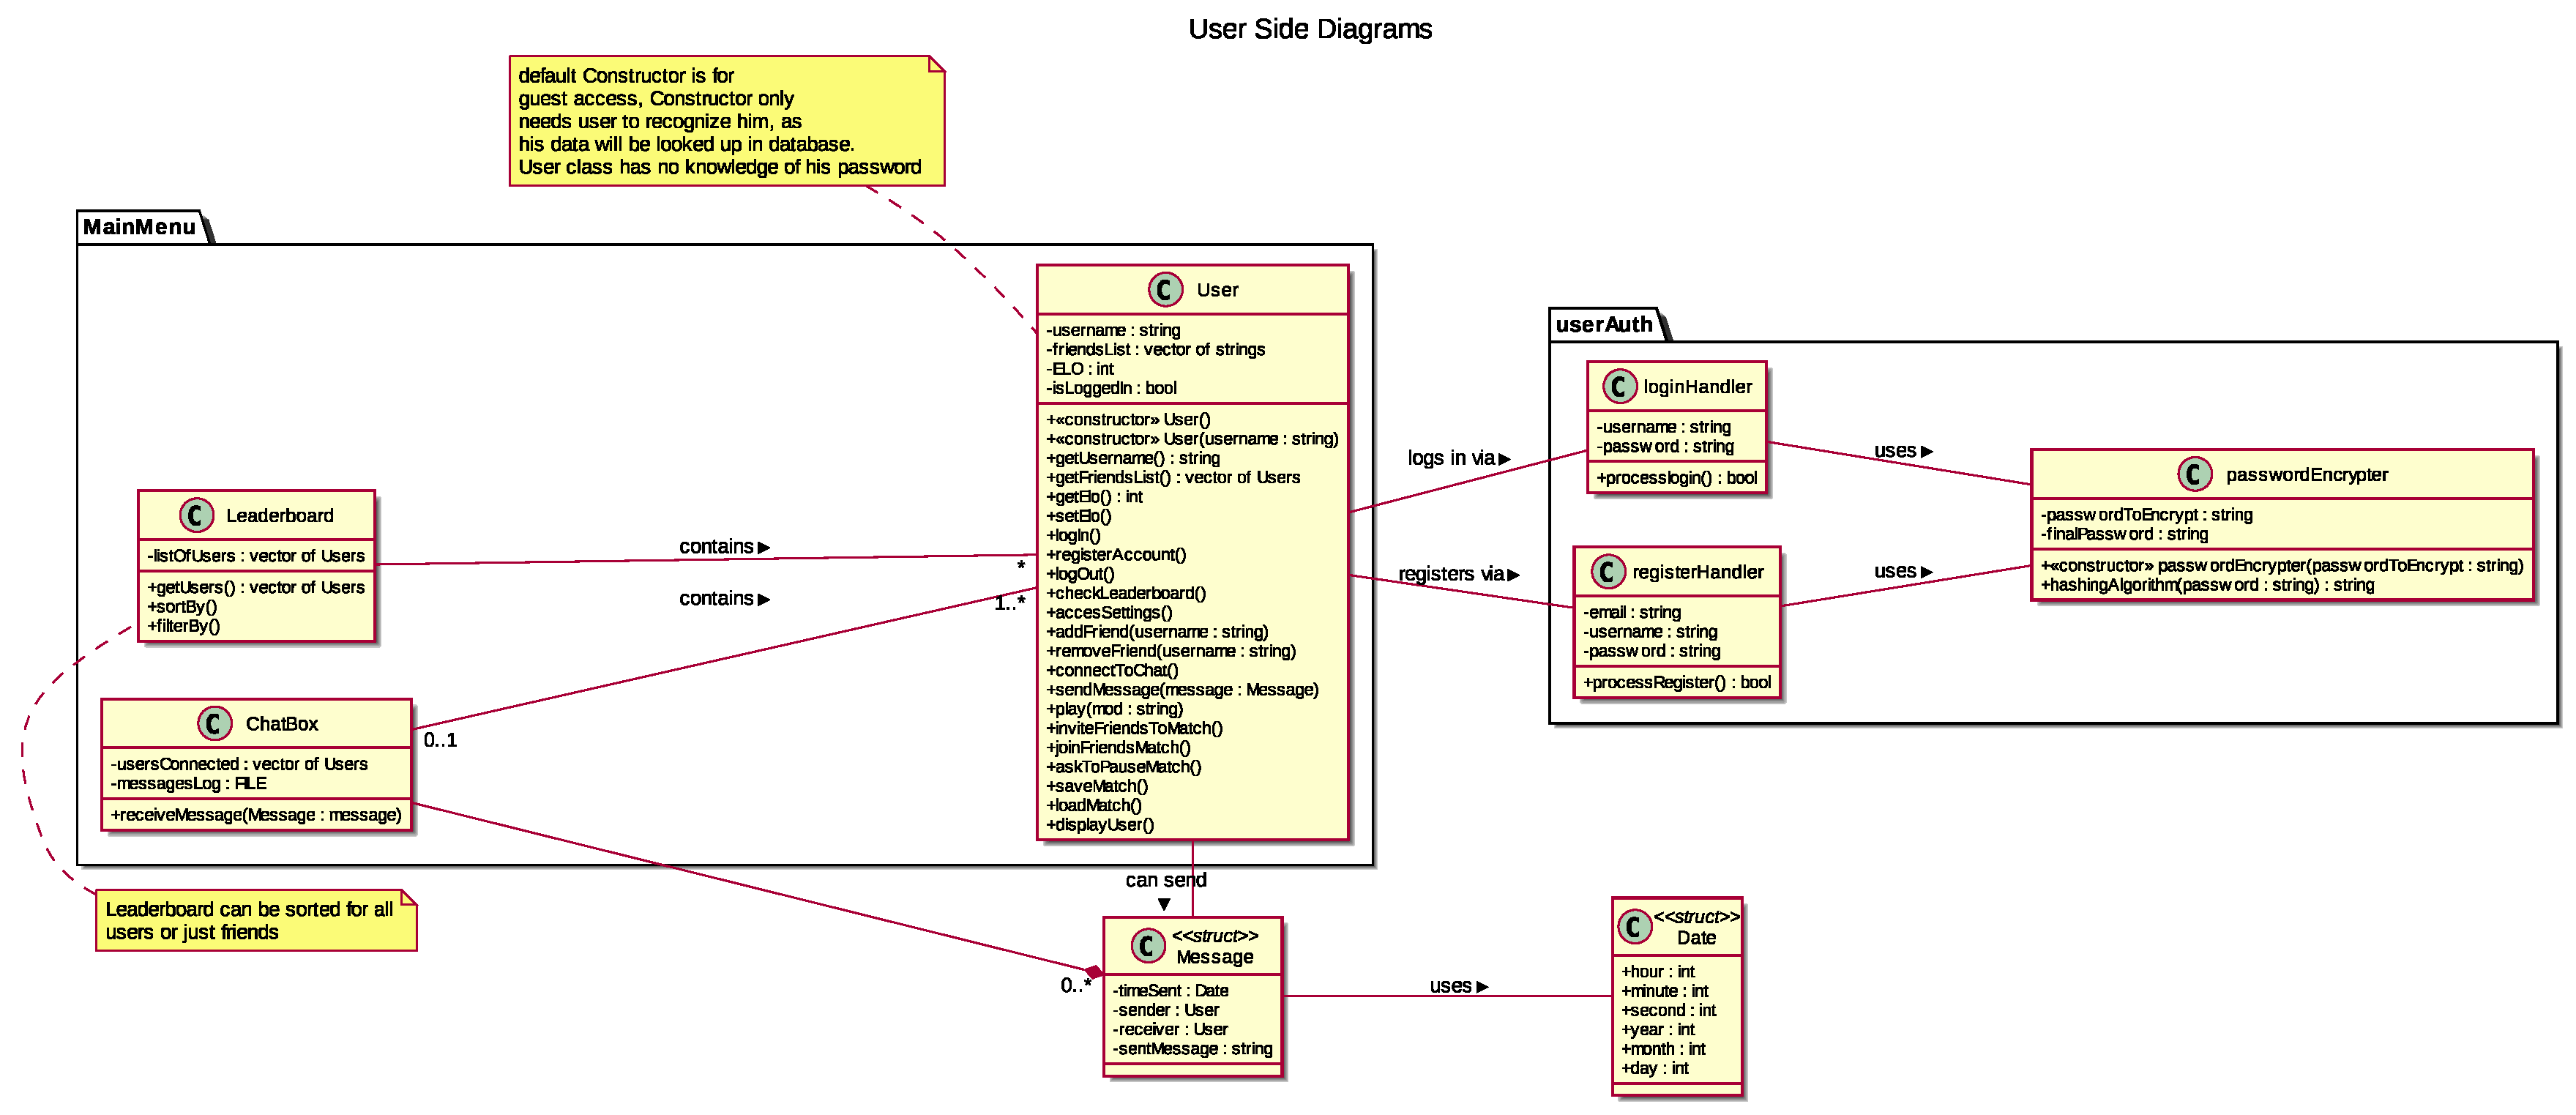
\includegraphics[width=\textwidth]{UserSideDiagrams.eps}}
    \addimg{img/6_UserSideDiagrams.eps}{width=\textwidth}{Diagrammes du côté utilisateur}{usrside}
        L'utilisateur entre dans le jeu comme une sorte de "Guest",
        ne pouvant pas utiliser l'interface
        Pour pouvoir utiliser les fonctionnalités de Quoridor, l'utilisateur doit se connecter
        à son compte ou en créer un s'il n'en a pas. Les deux evenements passeront à travers des "handlers", qui
        géreront les requetes en passant à travers un database et le Server. Après s'etre connecté.e, l'utilisateur aura accès à toutes les fonctionnalités
        que offre le logiciel (cfr. Sections 2 et 4).
    \subsubsection{Coté jeu}
        % \makebox[\textwidth]{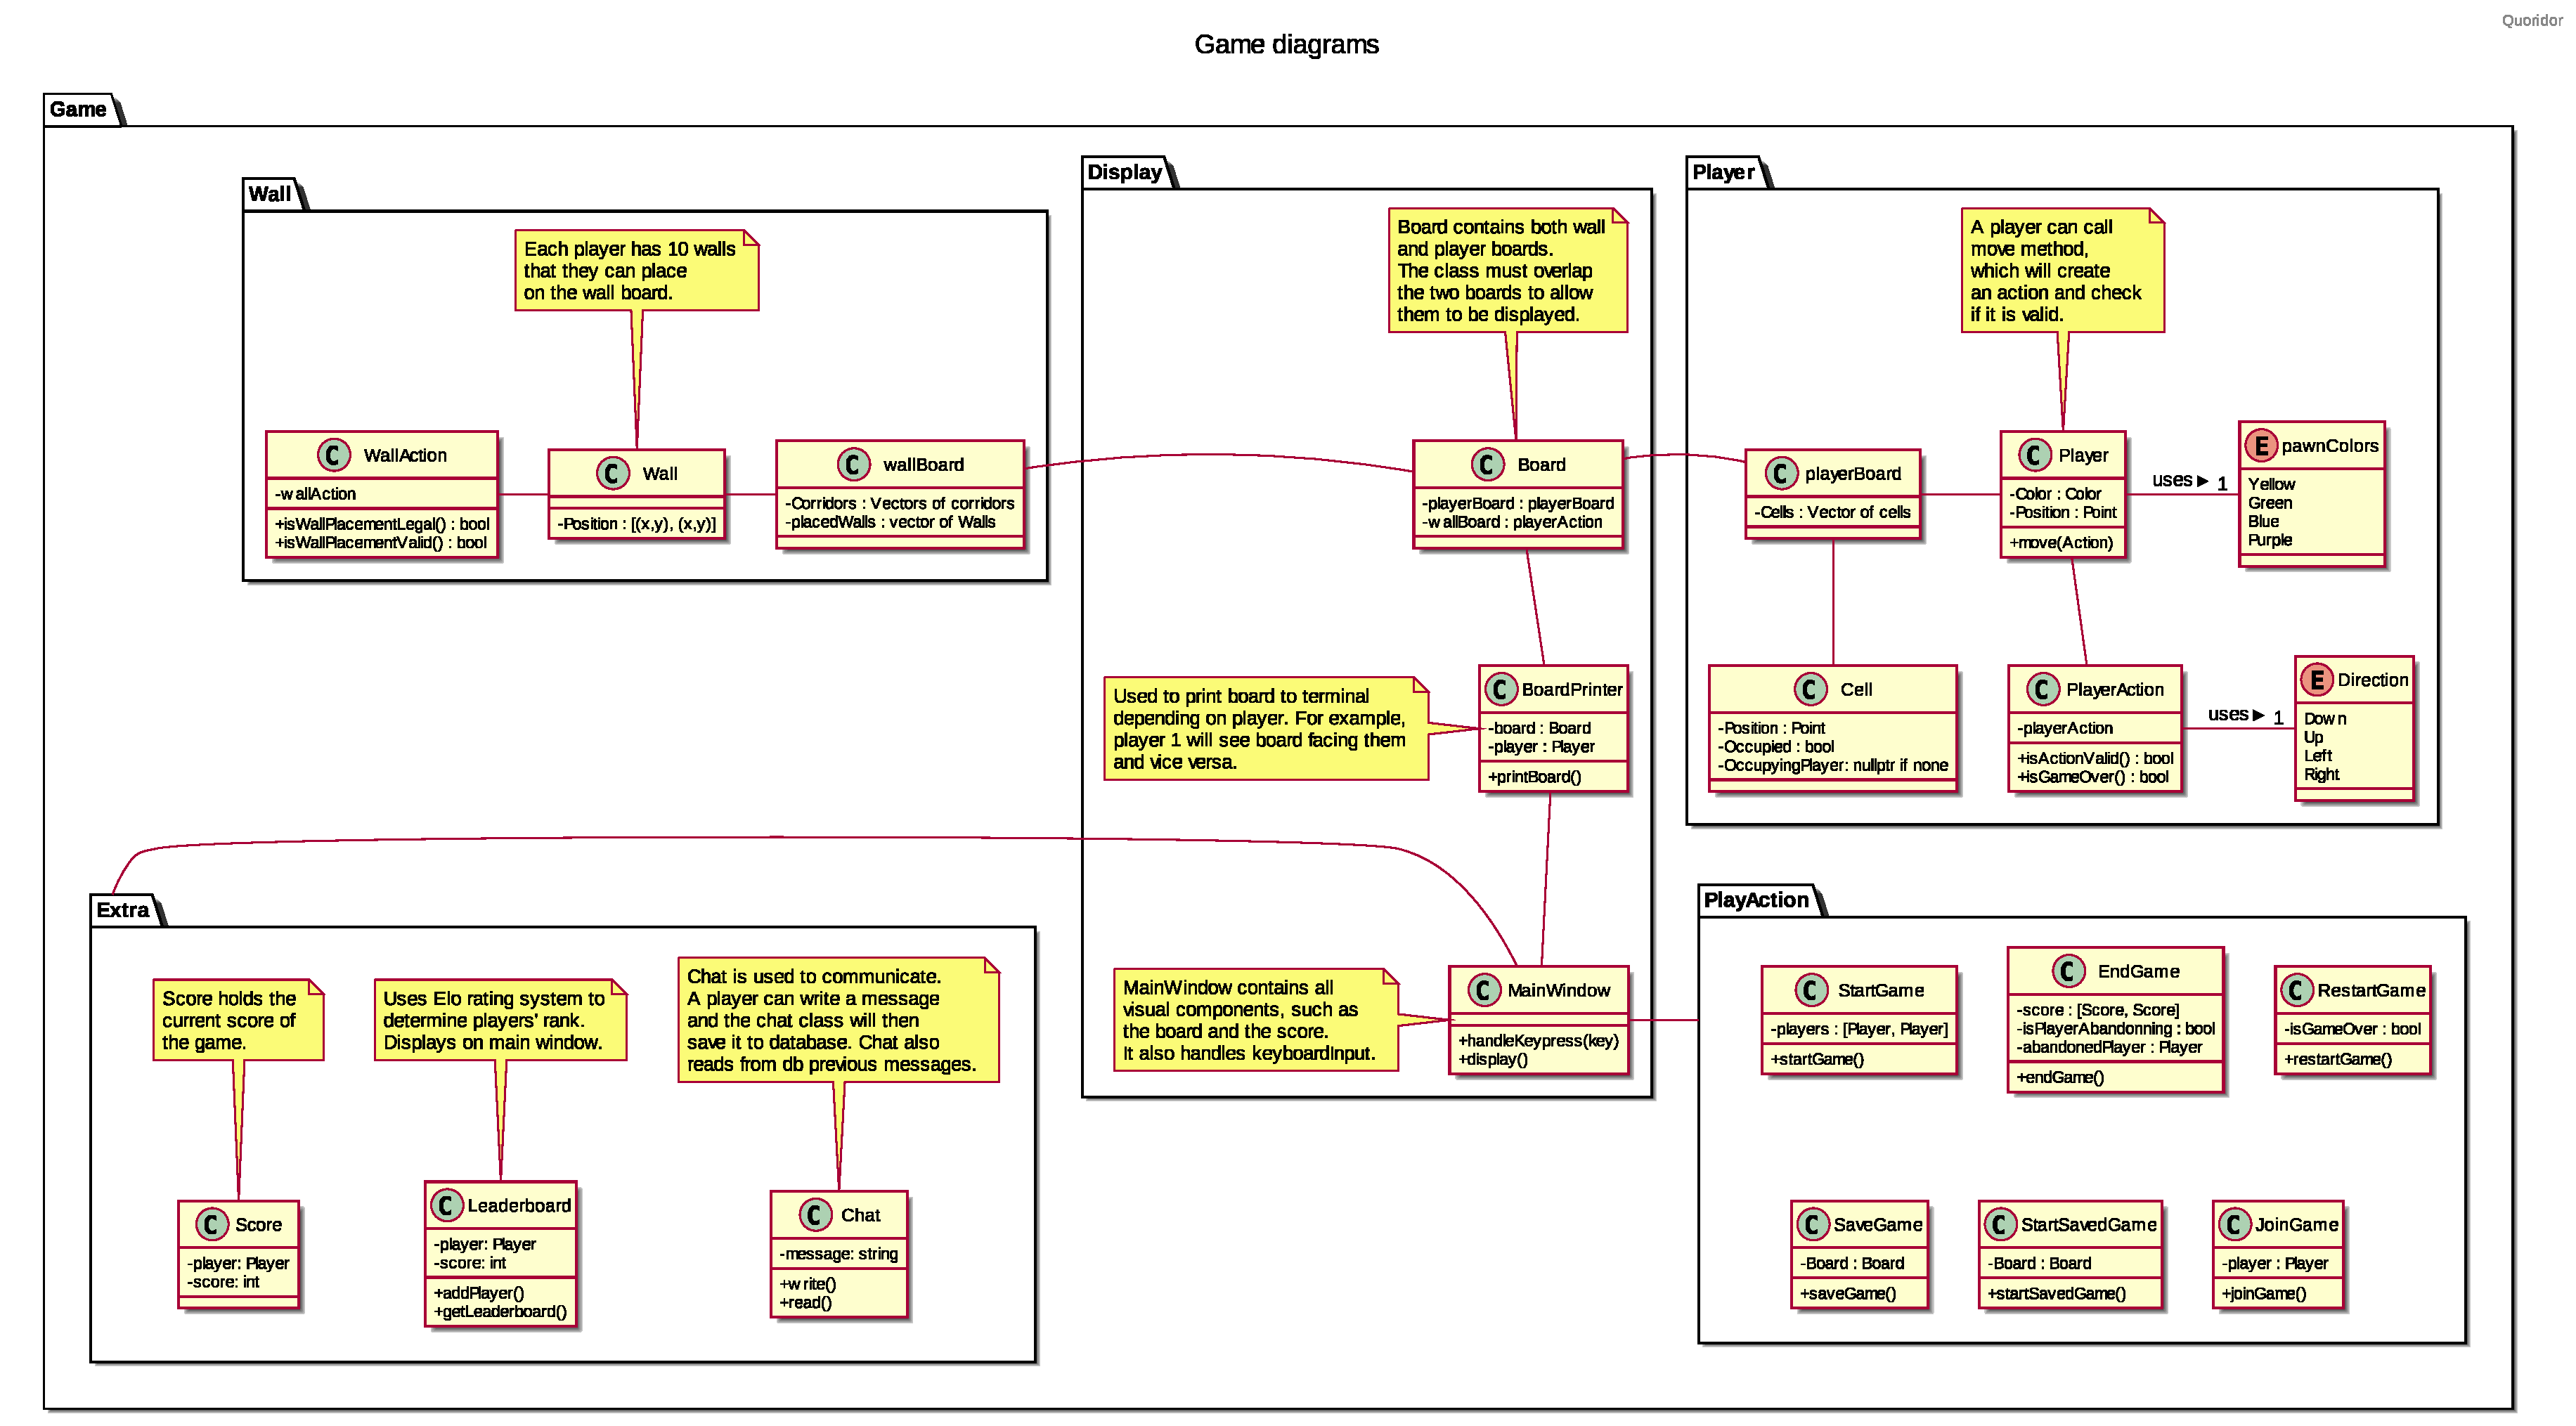
\includegraphics[width=\textwidth]{GameDiagrams.eps}} 
    \addimg{img/6_GameDiagrams.eps}{width=\textwidth}{Diagrammes de jeu}{gameside}
    


\subsection{Coté Serveur}

\addimg{img/6_ServerSideDiagram.eps}{width=\linewidth}{Diagramme du cote serveur}{serverside}

Le serveur gère la connexion ou l'enregistrement d'un client. 
Le gestionnaire de connexion vérifie la validité du nom d'utilisateur et
du mot de passe en vérifiant dans la base de donnée qu'il existe bien un utilisateur avec ce mot de passe. Il en informe ensuite le client.
Le gestionnaire d'enregistrement lui va vérifier la disponibilité du nom d'utilisateur. Si cela est valide, il crypte le mot de passe et enregistre les identifiants du client dans la base de donnée. Le serveur informe le client si l'enregistrement a bien eu lieu.

Le client peut envoyer et recevoir des messages.
Un message contient une chaîne de caractère entrée par l' utilisateur, les informations du receveur, de l'envoyeur ainsi que l'horodatage de l'envoie du message. Ce message sera enregistré dans la base de donnée. Le serveur informe les clients à chaque fois qu'un message est envoyé dans le chat.

Le serveur gère les actions du client sur le plateau.
Chaque client peut envoyer une action, le serveur vérifie la validité du coup et vérifie également si une partie est fini. Le serveur enregistre la partie dans la base de donnée.


\subsection{Fonctionnement du système}
        \subsubsection{Inscription}
        \addimg{img/6_Reg.eps}{width=\linewidth}{Register process}{regSeq}
        \subsubsection{Connexion}
        \addimg{img/6_Login.eps}{width=\linewidth}{Login process}{loginSeq}
        \subsubsection{Chat}
        \addimg{img/6_ChatSequence.eps}{width=\linewidth}{Chat process}{chatSeq}
        \subsubsection{Calcul du ELO}
        Pour comprendre comment fonctionne le matchmaking, il nous faut d'abord comprendre comment fonctionne le système de classement ELO, qui se résume en une phrase:
        \textit{"Le classement Elo est un système d’évaluation comparatif du niveau de jeu des joueurs d’échecs, de go ou d’autres jeux en un contre un."}\footnote{Wikipedia, Classement ELO} \\
        L'ELO est différent de modalité en modalité. \\
        Pour le calculer, nous n'allons pas développer un nouvel algorithme. Nous allons plutôt nous baser sur cet article \footnote{\href{https://metinmediamath.wordpress.com/2013/11/27/how-to-calculate-the-elo-rating-including-example/}{Metin's Media and Math, How To Calculate the Elo-Rating }}.
        Puisque le jeu Quoridor peut être joué par quatre joueur, il nous faut adapter le calcul afin que celui-ci reste équilibré. \\
        Supposons alors une première situation pour une partie en 1v1 avec les joueurs 1 et 2 dans l'ELO:
    \begin{center}
        r(1) = 1500 et r(2) = 1753
    \end{center}
    Nous allons tout d'abord calculer le \textit{transformed score} R(n) comme suit:
    \begin{equation}
        \begin{split}
            & R(1) = 10^{\frac{r(1)}{400}} = 5623,413 \\
            & R(2) = 10^{\frac{r(2)}{400}} = 24126,815 \\
        \end{split}
    \end{equation}

    Ensuite, nous calculons le \textit{expected score} E(n):
    \begin{equation}
        \begin{split}
            & E(1) = R(1) / ( R(1) + R(2)) = 5623,413 / (5623,413 + 24126,815) = 0,189 \\
            & E(2) = R(2) / ( R(1) + R(2)) = 24126,815 / (5623,413 + 24126,815) = 0,8109 \\
        \end{split}
    \end{equation}

    Définissons le \textit{actual score} pour les 2 joueurs:
    \begin{center}
        S(n) = 1 s'il gagne / 0 s'il perd
    \end{center}

    Calculons l'ELO final r'(n):
    Pour cela nous devons définir K: \\
    \textit{"This is called the K-factor and basically a measure of how strong a match will impact the players’ ratings.
    If you set K too low the ratings will hardly be impacted by the matches and very stable ratings (too stable) will occur.
    On the other hand, if you set it too high, the ratings will fluctuate wildly according to the current performance.
     Different organizations use different K-factors, there’s no universally accepted value. In chess the ICC uses a value of K = 32".}\footnote{\href{https://metinmediamath.wordpress.com/2013/11/27/how-to-calculate-the-elo-rating-including-example/}{Metin's Media and Math, How To Calculate the Elo-Rating }} \\
    Ici, nous supposons que le joueur 1 ait gagné.
    \begin{equation}
        \begin{split}
           & r'(1) = r(1) + K \cdot (S(1) - E(1)) = 1500 + 32 \cdot (1 - 0,189) = 1525,952 \\
           & r'(2) = r(2) + K \cdot (S(2) - E(2)) = 1753 + 32 \cdot (0-0,8109) = 1727,0512 \\
        \end{split}
    \end{equation}

    Les ELO finaux des deux joueurs seront :
    \begin{center}
        r(1) = 1526, +26 \ r(2) = 1727, -26
    \end{center}

    Supposons maintenant la partie se déroule entre 4 joueurs, 1, 2, 3 et 4:
    \begin{center}
        r(1) = 1700, r(2) = 1900, r(3) = 1500, r(4) = 1600
    \end{center}
    Comme avant, calculons les \textit{transformed scores}:
        \begin{equation}
            \begin{split}
                & R(1) = 10^{\frac{1700}{400}} = 17782,794 \\
                & R(2) = 10^{\frac{1900}{400}} = 56243,1325 \\
                & R(3) = 10^{\frac{1500}{400}} = 5623, 413  \\
                & R(4) = 10^{\frac{1600}{400}} = 10000 \\
            \end{split}
        \end{equation}
        Pour les \textit{expected scores} E(n) de chaque joueur, nous considérerons la moyenne pondérée des "transformed scores" R(m) des autres joueurs.
        Nous voulons que la moyenne soit pondérée afin de tenir compte de la différence entre les ELO des joueurs. Une disparité plus grande affectera
        de manière différente l'ELO final dans les cas d'une victoire ou d'une défaite.  \\
        Nous procéderons comme suit: \\
        Pour deux joueurs n et m: $\varepsilon = $ r(n) - r(m)  \\
        Nous considérons $< -100 \text{ et } > 100$ comme un écart significatif
            $$ \omega_{n, m} =
            \begin{cases}
                1 + \varepsilon \cdot 10^{-3}, & \text{si $\varepsilon \le -100$} \\
                1 - \varepsilon \cdot 10^{-3}, & \text{si $\varepsilon \ge 100$} \\
                1, & \text{si $-100 < \varepsilon < 100$ }\\
            \end{cases} $$
        
        E(1), E(2), E(3) et E(4) se calculeront comme suit, avec J le nombre de joueurs adversaires (3):
        \begin{equation}
            \begin{split}
                & E(1) = R(1) / [R(1) + (\dfrac{R(2) \cdot \omega_{1, 2} + R(3) \cdot \omega_{1, 3} + R(4) \cdot \omega_{1, 4}}{J})] = 0,394 \\
                & E(2) = R(2) / [R(2) + (\dfrac{R(1) \cdot \omega_{2, 1} + R(3) \cdot \omega_{2, 3} + R(4) \cdot \omega_{2,4} }{J})] = 0,872 \\
                & E(3) = R(3) / [R(3) + (\dfrac{R(1) \cdot \omega_{3, 1} + R(2) \cdot \omega_{3, 2} + R(4) \cdot \omega_{3,4} }{J})] = 0,131 \\
                & E(4) = R(4) / [R(4) + (\dfrac{R(1) \cdot \omega_{4, 1} + R(2) \cdot \omega_{4, 2} + R(3) \cdot \omega_{4,3} }{J})] = 0,232 \\
            \end{split}
        \end{equation}
        S(n) sera défini comme avant : 1 si le joueur a gagné, 0 s'il a perdu.

        Le calcul du ELO final r'(n) s'effectue de la même manière:
        \begin{equation}
            \begin{split}
                & r'(1) = r(1) + K \cdot (S(1) - E(1)) = 1719 \\
                & r'(2) = r(2) + K \cdot (S(2) - E(2)) = 1872 \\
                & r'(3) = r(3) + K \cdot (S(3) - E(3)) = 1495 \\
                & r'(4) = r(4) + K \cdot (S(4) - E(4)) = 1592 \\
            \end{split}
        \end{equation}

        L'ELO final pour chaque joueur correspondra alors à r'(n). \\
        Nous pouvons constater que les ELO finaux sont raisonnables si mis en rapport avec la disparité de l'ELO initiale. Les joueurs 3 et
        4 ne voient pas leur ELO diminuer d'une grande marge. En revanche, le joueur 2 qui possédait auparavant l'ELO le plus haut, constate une diminution de 28.

\section{Modes de jeu supplémentaires}
\begin{itemize}
    \item Timer : Chaque joueur aura un temps limité pour gagner sa partie. Lorsque c'est au tour d'un joueur de jouer, son temps s'épuise. Une fois son coup effectué, son timer se met en pause jusqu'à ce que ce soit à nouveau son tour de jouer. 
    \item Quoritris: Inspiré du jeu Tetris, ce mode propose aux joueurs de placer des murs de formes aléatoires sur le plateau. Les murs ont la possibilité de faire des rotations de 90 degrés sur eux-même.    
    \item Blinding Wall : Le mode de jeu des murs aveuglant se déroule comme une partie normale, excepté que les murs placés sur le plateau obstruent la vue des joueurs. Une fois un mur placé devant lui, le joueur ne voit plus rien de ce qui se passe derrière ce mur.
\end{itemize}
\section{Base de donnée}
Afin de réaliser ce projet, il est primordial pour le serveur de stocker les données continuellement et non pas seulement pendant l'exécution du programme. Pour ce faire, il est nécessaire d'utiliser une base de donnée. De ce fait, plusieurs choix s'offrent à nous.
Nous allons évaluer ces choix potentiels en prenant en compte leur utilité dans le cadre de ce projet.

\subsection{SQL}
Le \textit{relational data model} que SQL apporte, domine le type de base de données sur l'internet moderne. Ce modèle de stockage peut s'avérer utile dans le cadre de ce projet.

\subsubsection{SQLite}
SQLite permet d'implémenter rapidement et facilement ce modèle. En revanche, SQLite n'est pas idéal pour la gestion d'utilisateur et la concurrence puisque seulement un seul processus peut modifier la base de donnée à la fois.

\subsubsection{MySQL}
MySQL est l'implémentation de ce modèle la plus populaire. MySQL semble être un bon choix pour ce projet de part pour sa fiabilité mais aussi pour sa popularité qui entraînera donc une facilité lors de recherches à son sujet.

\subsubsection{PostgreSQL}
PostgreSQL est un choix solide puisqu'il a la plupart des mêmes avantages de MySQL mais a en plus la capacité de stocker plus de types de données nativement, tel que JSON, ce qui pourraient s'avérer très utile. Un inconvénient de PostgreSQL est que la performance au niveau de la mémoire n'est pas idéale mais cela ne devrait pas poser de problème vu que nous n'allons à priori pas gérer plusieurs milliers de joueurs à la fois.

\subsection{MongoDB et autre base de données NoSQL}
MongoDB est un modèle de base de donnée plus moderne se basant sur le NoSQL. MongoDB peut s'avérer être un bon choix grâce à sa grande flexibilité et sa rapidité. MongoDB est néanmoins moins populaire que SQL mais semble être un choix idéal pour ce projet.

\subsection{Fichier text}
Une autre méthode de stockage de données serait un simple fichier texte. Cela n'est pas idéal dû principalement au manque de structure que cela apporte.

\subsection{Décision}
La décision concernant la base de donnée n'a pas encore été faite mais à premier abord MongoDB et PostgreSQL semble être des choix idéals pour accomplir ce projet. Une base de données se basant sur l'un ou l'autre nécessitera néanmoins une grande part de travail pour leur intégration au serveur.
Il s'avèrera sûrement utile de faire tourner la base de donnée et le serveur dans des containers à l'aide de Docker par exemple afin de simplifier la reproduction du serveur sur d'autres machines.


% \section{Squellettes de code}

% \addcode{../src/resources/Board.h}{C++}{}
% \addcode{../src/resources/BoardPrinter.h}{C++}{}
% \addcode{../src/resources/Cell.h}{C++}{}
% \addcode{../src/resources/chatbox.h}{C++}{}
% \addcode{../src/resources/Chat.h}{C++}{}
% \addcode{../src/resources/const.h}{C++}{}
% \addcode{../src/resources/date.h}{C++}{}
% \addcode{../src/resources/EndGame.h}{C++}{}
% \addcode{../src/resources/JoinGame.h}{C++}{}
% \addcode{../src/resources/leaderboard.h}{C++}{}
% \addcode{../src/resources/LeaderBoard.h}{C++}{}
% \addcode{../src/resources/loginhandler.h}{C++}{}
% \addcode{../src/resources/Mainwindow.h}{C++}{}
% \addcode{../src/resources/message.h}{C++}{}
% \addcode{../src/resources/passwordencrypter.h}{C++}{}
% \addcode{../src/resources/PlayerAction.h}{C++}{}
% \addcode{../src/resources/PlayerBoard.h}{C++}{}
% \addcode{../src/resources/PlayerEnum.h}{C++}{}
% \addcode{../src/resources/Player.h}{C++}{}
% \addcode{../src/resources/Point.h}{C++}{}
% \addcode{../src/resources/registerhandler.h}{C++}{}
% \addcode{../src/resources/RestartGame.h}{C++}{}
% \addcode{../src/resources/SaveGame.h}{C++}{}
% \addcode{../src/resources/Score.h}{C++}{}
% \addcode{../src/resources/StartGame.h}{C++}{}
% \addcode{../src/resources/StartSavedGame.h}{C++}{}
% \addcode{../src/resources/user.h}{C++}{}
% \addcode{../src/resources/WallAction.h}{C++}{}
% \addcode{../src/resources/WallBoard.h}{C++}{}
% \addcode{../src/resources/Wall.h}{C++}{}

\end{document}
